\documentclass[unknownkeysallowed,final]{beamer}
\usetheme{RJH} %RJH}
\usepackage[orientation=landscape,size=a2,scale=1.4,debug]{beamerposter}
\usepackage[absolute,overlay]{textpos}
\setlength{\TPHorizModule}{1cm}
\setlength{\TPVertModule}{1cm}

\usepackage{amsmath,amsthm, amssymb, latexsym}
\usepackage{multirow}
\usepackage{rotating}

\usepackage{array,booktabs,tabularx}
\newcolumntype{Z}{>{\centering\arraybackslash}X} % centered tabularx columns
\newcommand{\pphantom}{\textcolor{ta3aluminium}} % phantom introduces a vertical space in p formatted table columns??!!
\newcommand{\vectornorm}[1]{\left|\left|#1\right|\right|}

\title{\normalsize{Efficient Techniques for Simulations of Kinetic Equations of Gas Dynamics}}
\author{\small{Craig Euler, \hspace{5mm} College of Science and Mathematics ,\hspace{5mm} California State University Northridge}}
\footer{}
\date{}
% \includegraphics[scale=.2]{CSUN_seal.png}}
















\begin{document}
\tiny{}
\begin{frame}{} 
	
	


	\begin{textblock}{19.5}(1,4)

\begin{block}{\small{Introduction}}
Numerical simulations of gas flows over sharp leading edges of air vehicles are challenging because they require the solution of model kinetic equations. These equations lead to stiff problems in regimes transitional from continuum to free molecular flow. The main difficulties in solving model kinetic equations include the loss of the conservation of mass, momentum, and energy, and low order convergence of solutions. Flows that are near continuum are well described by the Boltzmann equation with the BGK collision model:

% Boltzmann equation
\begin{equation*}
\label{ES-BGK}
\partial_{t} f(t, \vec{x}, \vec{u}) + \vec{v} \cdot \vec{\nabla}_{x} f(t, \vec{x}, \vec{v}) = \nu (f_{0} - f)
\end{equation*}
% use \ref{ES-BGK} or \eqref{ES-BGK} to get the reference for this equation

Where $f_{0}$ is the Maxwellian equilibrium distribution

% f0
\begin{equation*}
\label{f0}
f_{0} = f_{M} = \frac{\rho(t, \vec{x})}{\sqrt{(2 \pi RT(t, \vec{x}))^{3}}} \exp \left( -\frac{( \vec{v}- \vec{\bar{u}}(t, \vec{x}))^{2}}{2RT} \right)
\end{equation*}
% use \ref{f0} or \eqref{f0} to get the reference for this equation

\end{block}

\begin{block}{\small{Reduction to One Dimension}}
We assume that there is no mass transfer in the $y$ and $z$ directions (examples: gas between two parallel plates or in an infinitely wide pipe). In this case, the BGK equation reduces to

%A one dimensional reduction is performed on \eqref{ES-BGK} by assuming that no mass transfer occurs in two of the three directions in space, in this case $v_{2}$ and $v_{3}$. By considering the fallowing substitutions:

% f1
%\begin{equation*}
%\label{f1}
%f^{1} (t,x,v_{1}) = \int_{-\infty}^{\infty} \int_{-\infty}^{\infty} f(t, \vec{x}, \vec{v}) dv_{2} dv_{3}
%\end{equation*}
% use \ref{f1} or \eqref{f1} to get the reference for this equation

% f2
%\begin{equation*}
%\label{f2}
%f^{2} (t,x,v_{1}) = \int_{-\infty}^{\infty} \int_{-\infty}^{\infty} v_{2}^2 f(t, \vec{x}, \vec{v}) dv_{2} dv_{3}
%\end{equation*}
% use \ref{f2} or \eqref{f2} to get the reference for this equation

%then by integrating \eqref{ES-BGK} over all velocity space we are left with the following reduction with $j=1,2$:

% First PDE evolution equation for f1 and f2
\begin{equation*}
\label{bgk1d1}
\partial_{t} f^{1,2}(t,x,v) + v \partial_{x} f^{1,2}(t,x,v) = Q^{1,2}(f^{1,2},v)
\lefteqn{\hspace{20mm}(1)}
\end{equation*}

%Where

\begin{equation*}
\label{Q1}
Q^{1}(f^{1},v) = \nu \left( \frac{\rho(t, x)}{\sqrt{2 \pi RT(t, x)}} \exp \left( - \frac{(v - \bar{u})^{2}}{2RT} \right) - f^{1}(t, x, v) \right)
\end{equation*}

\begin{equation*}
\label{Q2}
Q^{2}(f^{2},v) = \nu \left( \rho(t, x) \sqrt{ \frac{RT(t, x)}{2 \pi}} \exp \left( - \frac{(v - \bar{u})^{2}}{2RT} \right) - f^{2}(t, x, v) \right)
\end{equation*}

%and

% Density in 1D
%\begin{equation*}
%\label{density_1d}
%\rho(t,x) = \int_{-\infty}^{\infty} f^{1}(t, x, v) dv_{1}
%\end{equation*}
% use \ref{density_1d} or \eqref{density_1d} to get the reference for this equation

% Momentum in 1D
%\begin{equation*}
%\label{momentum_1d}
%\bar{u}(t,x) = \frac{1}{\rho(t,x)}\int_{ -\infty}^{\infty} v_{1} f^{1}(t, x, v_{1}) dv_{1}
%\end{equation*}
% use \ref{momentum_1d} or \eqref{momentum_1d} to get the reference for this equation

% Temperature in 1D
%\begin{equation*}
%\label{temperature_1d}
%T(t,x) = \frac{1}{3R \rho(t,x)} \int_{-\infty}^{\infty} \left[ (v_{1} - \bar{u})^{2} f^{1}(t, x, v_{1}) + 2 f^{2}(t, x, v_{1}) \right]dv_{1}
%\end{equation*}
% use \ref{temperature_1d} or \eqref{temperature_1d} to get the reference for this equation

Where $f^{1} = \int f \, dv \, dw $ can be a reduced molecular distribution function and $f^{2} = \int v^{2} f \, dv \, dw $.
\end{block}

\begin{block}{\small{DG Velocity Discretization}}
We let $V=[v_{L}, v_{R}]$ be an interval large enough so that the first moment integrals of the distribution function outside of it are negligible and let it be partitioned into subintervals $I_{i}=[v_{i-1/2},v_{1+1/2}]$. Let $\chi_{p}$ and $\omega_{p}$, $p=1,\ldots,s$ denote the nodes and weights of the Gaussian quadrature of order $P$ on the interval $[-1,1]$. On $[v_{i-1/2},v_{i+1/2}]$ we define

\begin{equation*}
\label{Chi}
\chi_{p,i} = \frac{v_{i+1/2} + v_{i-1/2}}{2} + \chi_{p}\frac{v_{i+1/2} - v_{i-1/2}}{2}.
\end{equation*}
% use \ref{Chi} or \eqref{Chi} to get the reference for this equation

Our basis functions $\varphi_{p,i}(v)$ are
\begin{equation*}
\varphi_{p,i}(v) = \prod\limits_{q=1,s \atop q \neq p} \frac{v-\chi_{q,i}}{\chi_{p,i} - \chi_{q,i}}.
\end{equation*}
\end{block}

	\end{textblock}

	\begin{textblock}{18}(21.8,4)

 \begin{block}{\small{}}
Notice that basis functions satisfy the orthogonality properties

\begin{equation*}
\int_{v_{i-1/2}}^{v_{i+1/2}} \phi_{p,i}(v) \phi_{q,i}(v) = \frac{\Delta v_{i}}{2} \omega_{p} \delta_{p,q}
\end{equation*}

and

\begin{equation*}
\int_{v_{i-1/2}}^{v_{i+1/2}} v \phi_{p,i}(v) \phi_{q,i}(v) = \frac{\Delta v_{i}}{2} \chi_{p,q} \omega_{p} \delta_{p,q},
\end{equation*}

where $\delta_{p,q}$ is the Kronecker delta function.

The discrete velocity approximations of $f^{1,2}(t,x,v)$ are defined by

\begin{equation*}
\label{eq0x}
f^{1,2}(t,x,v)=\sum_{p=1} ^{s} f_{p,i}^{1,2}(t,x) \varphi_{p,i}(v).
\end{equation*}
% use \ref{base} or \eqref{base} to get the reference for this equation
Substituting the discrete velocity approximations into (1) and multiplying by our basis functions and integrating through velocity, after simplification we arrive at

\begin{equation*}
\label{eqint}
\partial_{t} f_{q,i}^{1,2}(t,x) + \chi_{p,i} \partial_{x} f_{q,i}^{1,2}(t,x) = Q^{1,2}(f^{1,2},\chi_{p,i}).
\end{equation*}

Notice that these equations have the form of a first order symmetric hyperbolic system.

\end{block}

\begin{block}{\small{Clawpack}}
Clawpack is a software package developed by LeVeque et al [1]. It is designed to provide solutions to Hyperbolic PDEs in 1 and 2 dimensions and of first or second orders. Current implementations of Clawpack include Geoclaw for Tsunami modelling and other geophysical flows. In our implementation, we seek to extend Clawpack to use for the solution of the model Boltzmann equations.
\end{block}

\begin{block}{\small{One Dimensional Heat Transfer}}
Nitrogen gas at 300K between two infinitely long parallel plates. The plate on the left is at 0m and is heated to 1000K. The plate on the right is at 0.1m and is heated to 300K. At 0.03 seconds the solution is observed to be near steady state.\\[2mm]
Our first experiment is to study the relative error in the total mass. The number of cells in space ranged from 10-100 and the number of cells through velocity ranged from 6 to 16 with a scheme order of 10 for velocity approximation.
We observed by varying the number of velocity cells we can reduce the error to a factor of $10^{-10}$. It is observed that varying the number of cells in the spatial variable $x$ has little effect on the conservation of mass as seen in the table below.

\end{block}
	\end{textblock}

	\begin{textblock}{17.3}(41,4)

\begin{block}{\small{}}

\begin{center}
	\begin{tabular}{ cc || c | c | c | c | c | c | c | c | c | r |}

& & \multicolumn{4}{| c |}{Number of velocity cells}\\
& & 6 & 8 & 12 & 16\\ \hline \hline
\multirow{10}{*}{\begin{sideways}{Number of spatial cells}\end{sideways}}
& 10 & 5.30E-07 & 1.83E-09 & 1.26E-09 & 2.16E-10\\ \cline{2-6}
& 20 & 5.33E-07 & 1.34E-09 & 7.81E-10 & 4.33E-10\\ \cline{2-6}
& 30 & 5.24E-07 & 1.44E-08 & 1.02E-08 & 9.34E-09\\ \cline{2-6}
& 40 & 5.33E-07 & 2.53E-09 & 7.89E-10 & 6.15E-10\\ \cline{2-6}
& 50 & 5.34E-07 & 2.12E-09 & 1.26E-09 & 3.06E-11\\ \cline{2-6}
& 60 & 5.54E-07 & 1.63E-08 & 1.93E-08 & 2.02E-08\\ \cline{2-6}
& 70 & 5.13E-07 & 2.25E-08 & 1.94E-08 & 1.93E-08\\ \cline{2-6}
& 80 & 5.34E-07 & 3.18E-09 & 2.73E-10 & 1.19E-09\\ \cline{2-6}
& 90 & 5.25E-07 & 1.24E-08 & 9.60E-09 & 9.79E-09\\ \cline{2-6}
& 100 & 5.33E-07 & 2.54E-09 &  5.10E-10 & 1.14E-10\\ \hline

\hline
	\end{tabular}
\end{center}

The convergence of the L2 norm of the error in macroparameters with respect to the resolution in the spatial variable can be seen in the table below. The solutions are compared to solutions on 1000 cells. The velocity discretization is by a scheme of order 10 on 10 velocity cells.

\begin{center}
	\begin{tabular}{ lc || c | c | c | c |}

& & \multicolumn{4}{| c |}{Number of spatial cells}\\
& & 50 & 100 & 150 & 200\\ \hline \hline
& Density & 0.03054 & 0.01737 & 0.01198 & 0.008234\\ \cline{2-6}
& Momentum & 17.06 & 8.383 & 5.368 & 3.842\\ \cline{2-6}
& Temperature & 0.03967 & 0.02408 & 0.01652 & 0.01062\\ \hline

\hline
	\end{tabular}
\end{center}



\end{block}

\begin{block}{\small{Steady State Solution}}
\begin{center}
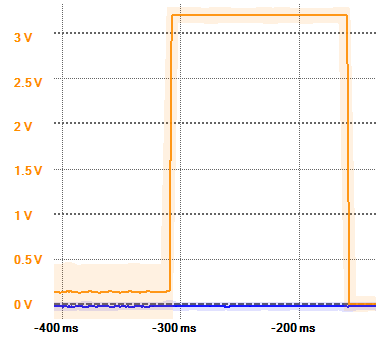
\includegraphics[scale=.75]{reference_pulse_32Hz_4sec_8downsample_2.png}
\end{center}
\end{block}

\begin{block}{\small{References}}
% http://depts.washington.edu/clawpack/users-4.6/about.html#authors
[1] R. J. LeVeque, M. J. Berger, et. al., Clawpack Software 4.5.1, www.clawpack.org, June 2011
\end{block}

	\end{textblock}

\end{frame}
\end{document}
